\documentclass[11pt]{article}
\usepackage[utf8]{inputenc}
\usepackage[a4paper,margin=0.85in]{geometry}
\usepackage{amsmath,amssymb,amsthm}
\usepackage{enumitem,parskip,hyperref,xcolor,fancyhdr,tikz,graphicx,eso-pic,titlesec,listings}
\graphicspath{{../}}
\definecolor{kcpc-text}{RGB}{20,20,20}
\definecolor{kcpc-muted}{RGB}{90,90,90}
\definecolor{kcpc-red}{RGB}{176,0,0}
\pagestyle{fancy}\fancyhf{}
\lhead{\textcolor{kcpc-text}{\small\bfseries Solutions}}
\rhead{\textcolor{kcpc-muted}{\small Week 3}}
\cfoot{\textcolor{kcpc-muted}{\small KCPC}}
\renewcommand{\headrulewidth}{0.4pt}
\renewcommand{\headrule}{\hbox to\headwidth{\color{kcpc-red}\leaders\hrule height \headrulewidth\hfill}}
\setlength{\headheight}{28pt}
\AddToShipoutPictureBG{\begin{tikzpicture}[remember picture,overlay]
  \node[opacity=0.035,at=(current page.center)]{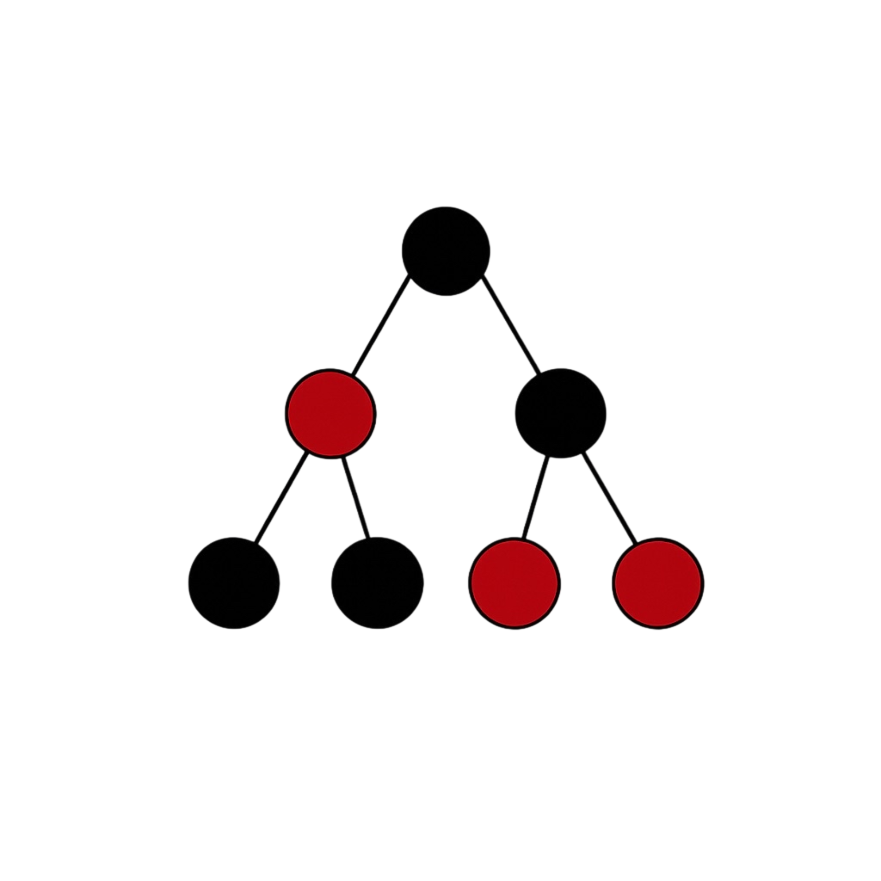
\includegraphics[width=0.38\paperwidth]{kcpc-logo.png}};
\end{tikzpicture}}
\titleformat{\section}{\large\bfseries\color{kcpc-red}}{\thesection}{1em}{}
\newcommand{\insight}[1]{\par\medskip\noindent\textbf{Key insight:} #1}
\lstset{basicstyle=\ttfamily\footnotesize,breaklines=true,columns=fullflexible,keepspaces=true,frame=single,showstringspaces=false}
\title{KCPC Week 3 Solutions\\The Lambda Calculus: Functions, Computation, and Numbers}
\author{}\date{}

\begin{document}
\maketitle\thispagestyle{fancy}

These solutions accompany all 12 problems. Equalities $\equiv_\beta$ mean beta-convertibility (up to alpha-renaming), not necessarily one reduction step. Every named function is a shorthand for a \emph{closed pure lambda term}. Python and C++ snippets demonstrate the same behaviour; the proofs establish correctness for arbitrary terms, beyond those executable examples.

\section{Foundational warm-ups}

\subsection*{1. Terms and parentheses}
\insight{An abstraction binds its entire body; application groups to the left.}
The full grammar writes the term as
\[(\lambda x.(\lambda y.(x(yz)))).\]
$\mathrm{FV}(yz)=\{y,z\}$, $\mathrm{FV}(x(yz))=\{x,y,z\}$, and removing $y$ and then $x$ under the two abstractions gives $\mathrm{FV}=\{z\}$. The root of $\lambda x.xy$ is an abstraction; its body $(xy)$ is an application.

\subsection*{2. Free variables and substitution}
\insight{Binding removes a variable from the free-variable set, not from the term.}
By structural definition,
\[\mathrm{FV}(x)=\{x\},\quad \mathrm{FV}(MN)=\mathrm{FV}(M)\cup\mathrm{FV}(N),\quad
  \mathrm{FV}(\lambda x.M)=\mathrm{FV}(M)\setminus\{x\}.\]
Thus $\mathrm{FV}((\lambda x.M)N)=(\mathrm{FV}(M)\setminus\{x\})\cup\mathrm{FV}(N)$.
For $(\lambda x.xy)z$ this is $(\{x,y\}\setminus\{x\})\cup\{z\}=\{y,z\}$. The $x$ in $xy$ lies inside $\lambda x$ and is bound by it; substitution for a different free $x$ cannot reach that occurrence.

\subsection*{3. Alpha conversion and capture}
\insight{A legal rename preserves which binder owns each occurrence.}
Rename the outer $x$ to fresh $u$, and the inner $y$ to fresh $v$, obtaining $\lambda u.\lambda v.uv$. By contrast, $\lambda y.\lambda y.yy$ binds both occurrences of $y$ at the inner binder; the first term has one occurrence belonging to each binder. Alpha-renaming cannot change that ownership.
For beta reduction, first rename the inner binder:
\[(\lambda x.\lambda y.x)y\equiv_\alpha(\lambda x.\lambda z.x)y\to_\beta\lambda z.y.\]
$y$ remains free. The incorrect $\lambda y.y$ binds it and has no free variables, so cannot be the same result.

\subsection*{4. Identity and constant functions}
\insight{An unused bound argument vanishes when its binder is applied.}
\[IA=(\lambda x.x)A\to_\beta A,\qquad
  KAB=(\lambda x.\lambda y.x)AB\to_\beta(\lambda y.A)B\to_\beta A,\]
\[FAB=(\lambda x.\lambda y.y)AB\to_\beta(\lambda y.y)B\to_\beta B.\]
Both selectors require two beta steps. In particular $KI\,I\to_\beta(\lambda y.I)I\to_\beta I$. If the substituted argument has free variables, alpha-rename an inner binder first as in Problem 3.

\subsection*{5. Currying and composition}
\insight{Applying one argument returns a function awaiting the next.}
\[Cfga=(\lambda f.\lambda g.\lambda x.f(gx))fga
  \to_\beta(\lambda g.\lambda x.f(gx))ga
  \to_\beta(\lambda x.f(gx))a\to_\beta f(ga).\]
Each abstraction takes one input. $CIIa\to_\beta^* I(Ia)\to_\beta^* a$. Also $CII\to_\beta^*\lambda x.I(Ix)\to_\beta^*\lambda x.x=I$. Reductions under abstractions are allowed when proving beta-convertibility.

\textbf{Executable illustration (Python):}
\begin{lstlisting}[language=Python]
I = lambda x: x
K = lambda x: lambda y: x
F = lambda x: lambda y: y
C = lambda f: lambda g: lambda x: f(g(x))
assert (I(7), K(7)(8), F(7)(8), C(I)(I)(7)) == (7, 7, 8, 7)
\end{lstlisting}
\textbf{The same warm-ups in C++17:}
\begin{lstlisting}[language=C++]
#include <cassert>
int main() {
    auto I = [](int x) { return x; };
    auto K = [](int x) { return [x](int) { return x; }; };
    auto F = [](int) { return [](int y) { return y; }; };
    auto C = [](auto f) {
        return [f](auto g) { return [f, g](int x) { return f(g(x)); }; };
    };
    assert(I(7) == 7 && K(7)(8) == 7 && F(7)(8) == 8);
    assert(C(I)(I)(7) == 7);
}
\end{lstlisting}
These functions illustrate application with integer inputs; integers here belong to the host languages, not to the pure calculus.

\section{Linked ideas: proofs and encodings}

\subsection*{6. Boolean selectors}
\insight{A Boolean is a function that selects one of two branches.}
Let $\mathrm{T}=\lambda a.\lambda b.a$ and $\mathrm{F}=\lambda a.\lambda b.b$. Choose
\[\mathrm{AND}=\lambda p.\lambda q.p\,q\,\mathrm{F},\qquad
  \mathrm{OR}=\lambda p.\lambda q.p\,\mathrm{T}\,q,\qquad
  \mathrm{NOT}=\lambda p.p\,\mathrm{F}\,\mathrm{T}.\]
All are closed after expanding abbreviations. From $\mathrm{T}ab\to_\beta^*a$ and $\mathrm{F}ab\to_\beta^*b$ we get the complete truth tables:
\[\begin{array}{c|c|c|c}
 p&q&\mathrm{AND}\,p\,q&\mathrm{OR}\,p\,q\\\hline
 \mathrm{T}&\mathrm{T}&\mathrm{T}&\mathrm{T}\\
 \mathrm{T}&\mathrm{F}&\mathrm{F}&\mathrm{T}\\
 \mathrm{F}&\mathrm{T}&\mathrm{F}&\mathrm{T}\\
 \mathrm{F}&\mathrm{F}&\mathrm{F}&\mathrm{F}
\end{array}\]
For both rows with $p=\mathrm{T}$, AND returns $q$ and OR returns $\mathrm{T}$; for both rows with $p=\mathrm{F}$, AND returns $\mathrm{F}$ and OR returns $q$. This proves every row independently of variable names. Also $\mathrm{NOT}\,\mathrm{T}\to_\beta^*\mathrm{F}$ and $\mathrm{NOT}\,\mathrm{F}\to_\beta^*\mathrm{T}$. Applying a selector to arbitrary $a$ and $b$ acts as a conditional without new syntax.

\subsection*{7. Church numerals and successor}
\insight{A numeral is an iterator, not an integer literal.}
\[\overline0=\lambda f.\lambda x.x,\qquad
  \overline1=\lambda f.\lambda x.fx,\qquad
  \overline2=\lambda f.\lambda x.f(fx).\]
Set $\mathrm{SUCC}=\lambda n.\lambda f.\lambda x.f(nfx)$. Expanding $\overline n$ gives
\[\mathrm{SUCC}\,\overline n\to_\beta^*\lambda f.\lambda x.f(\overline n f x)
\to_\beta^*\lambda f.\lambda x.f(f^n(x))=\overline{n+1}.\]
By the recursive definition of $f^n$, this holds for every $n\ge0$ (base $n=0$: $f(x)$; inductive step adds one outer $f$). In particular $\overline2\,g\,a\to_\beta(\lambda x.g(gx))a\to_\beta g(ga)$.

\subsection*{8. Arithmetic as iteration}
\insight{Addition concatenates iterations; multiplication composes iterators.}
Take
\[\mathrm{ADD}=\lambda m.\lambda n.\lambda f.\lambda x.m f(n f x),\qquad
  \mathrm{MUL}=\lambda m.\lambda n.\lambda f.m(n f),\qquad
  \mathrm{POW}=\lambda m.\lambda n.\lambda f.\lambda x.n m f x.\]
For arbitrary $f,x$, ADD yields $f^m(f^n(x))=f^{m+n}(x)$, where the identity follows by induction on $m$. MUL yields $(f^n)^m(x)=f^{mn}(x)$, by induction on $m$ using $n(m+1)=nm+n$. Finally $\overline n\,\overline m\,f\,x$ iterates the iterator $\overline m$ a total of $n$ times, applying $f$ $m^n$ times. At $n=0$ it yields $fx$, including $0^0=1$ under the stated convention. The outer $\lambda f.\lambda x$ in POW ensures that even for $n=0$ the resulting term is beta-convertible to the \emph{canonical} numeral $\overline1$: without this eta expansion $\overline0\,\overline m\to_\beta\lambda x.x$, which is not beta-convertible to $\overline1$.

\textbf{Numeral iteration in Python:}
\begin{lstlisting}[language=Python]
def numeral(n):
    def apply(f):
        def run(x):
            for _ in range(n):
                x = f(x)
            return x
        return run
    return apply

def succ(n): return lambda f: lambda x: f(n(f)(x))
def add(m, n): return lambda f: lambda x: m(f)(n(f)(x))
def mul(m, n): return lambda f: m(n(f))
value = lambda church: church(lambda x: x + 1)(0)
assert [value(numeral(0)), value(succ(numeral(2))),
        value(add(numeral(2), numeral(3))),
        value(mul(numeral(2), numeral(3)))] == [0, 3, 5, 6]
\end{lstlisting}

\textbf{The same encodings in C++17:}
\begin{lstlisting}[language=C++]
#include <cassert>
#include <functional>
using Fn = std::function<int(int)>;
using Church = std::function<Fn(Fn)>;
Church numeral(int n) {
    return [n](Fn f) -> Fn {
        return [n, f](int x) {
            for (int i = 0; i < n; ++i) x = f(x);
            return x;
        };
    };
}
Church succ(Church n) {
    return [n](Fn f) -> Fn {
        return [n, f](int x) { return f(n(f)(x)); };
    };
}
Church add(Church m, Church n) {
    return [m, n](Fn f) -> Fn {
        return [m, n, f](int x) { return m(f)(n(f)(x)); };
    };
}
Church mul(Church m, Church n) {
    return [m, n](Fn f) -> Fn { return m(n(f)); };
}
int main() {
    auto value = [](Church c) { return c([](int x) { return x + 1; })(0); };
    assert(value(numeral(0)) == 0);
    assert(value(succ(numeral(2))) == 3);
    assert(value(add(numeral(2), numeral(3))) == 5);
    assert(value(mul(numeral(2), numeral(3))) == 6);
}
\end{lstlisting}
The iterated \texttt{int} functions are small executable observations; the preceding equational argument proves the identities for any $f$ and $x$.

\subsection*{9. Subtraction by state threading}
\insight{To remember the previous numeral, iterate a pair of consecutive numerals.}
For a pair $p=\langle a,b\rangle$, the selector laws give $\mathrm{FIRST}\,p\equiv_\beta a$ and $\mathrm{SECOND}\,p\equiv_\beta b$. Thus $\mathrm{STEP}\langle a,b\rangle\equiv_\beta\langle b,\mathrm{SUCC}\,b\rangle$.
Let $P_n=\mathrm{STEP}^n\langle\overline0,\overline0\rangle$. $P_0=\langle\overline0,\overline0\rangle$, which matches $\max(-1,0)=0$. For $n=0$, $P_1=\langle\overline0,\overline1\rangle$. If $n\ge1$ and $P_n\equiv_\beta\langle\overline{n-1},\overline n\rangle$, then $P_{n+1}\equiv_\beta\langle\overline n,\overline{n+1}\rangle$. This completes induction, including the exceptional first step.
Since a Church numeral iterates a function,
\[\mathrm{PRED}=\lambda n.\mathrm{FIRST}\,(n\,\mathrm{STEP}\,(\mathrm{PAIR}\,\overline0\,\overline0))\]
represents $\max(n-1,0)$; in particular PRED$\,\overline0\equiv_\beta\overline0$. Set $\mathrm{SUB}=\lambda m.\lambda n.n\,\mathrm{PRED}\,m$. Induction on $n$ proves that $n$ applications of truncated predecessor give $\max(m-n,0)$, including $m<n$ and $m=0$.

\subsection*{10. Logic meets numbers}
\insight{Iterators can repeatedly update truth values as well as numbers.}
Let $\mathrm{ISZERO}=\lambda n.n\,(\lambda z.\mathrm{F})\,\mathrm{T}$.
For zero, there are no updates, so the answer is T. For $n+1$ there is at least one application of the constant-F function, and every subsequent application stays F; induction on $n$ proves the claim.
Let $\mathrm{EVEN}=\lambda n.n\,\mathrm{NOT}\,\mathrm{T}$. Its output starts at T and alternates T/F after each step. Base $n=0$ is T; if the claim holds for $n$, NOT flips the answer for $n+1$, proving parity by induction. Finally SUB$\,\overline m\,\overline n$ is zero iff $m\le n$, so ISZERO of that term selects T exactly in that case. This is a comparison on natural-number encodings, not an equality test on arbitrary lambda terms.

\textbf{Optional slide challenge (division).} Define $\mathrm{GE}=\lambda a.\lambda b.\mathrm{ISZERO}(\mathrm{SUB}\,b\,a)$, selecting T iff $a\ge b$, and let $\mathrm{IF}=\lambda c.\lambda a.\lambda b.cab$. For a fixed divisor $d$, define the closed-after-application step
\[\begin{aligned}
  \mathrm{DSTEP}={}&\lambda d.\lambda p.
    \mathrm{IF}\,(\mathrm{GE}\,(\mathrm{SUCC}(\mathrm{SECOND}\,p))\,d)\\
  &\quad(\mathrm{PAIR}\,(\mathrm{SUCC}(\mathrm{FIRST}\,p))
                 (\mathrm{SUB}\,(\mathrm{SUCC}(\mathrm{SECOND}\,p))\,d))\\
  &\quad(\mathrm{PAIR}\,(\mathrm{FIRST}\,p)
                 (\mathrm{SUCC}(\mathrm{SECOND}\,p))).
\end{aligned}\]
Set
\[\mathrm{DIV}=\lambda m.\lambda d.
    (\mathrm{ISZERO}\,d)\,\overline0\,
    (\mathrm{FIRST}\,(m\,(\mathrm{DSTEP}\,d)\,(\mathrm{PAIR}\,\overline0\,\overline0))).\]
For $d>0$, induction on the number $k$ of processed iterations shows that the state is $\langle\overline{\lfloor k/d\rfloor},\overline{k\bmod d}\rangle$. At $k=0$ it is $\langle0,0\rangle$. If the remainder $r<d-1$, the next step increments $r$; if $r=d-1$, it increments the quotient and subtracts $d$ from $r+1=d$, resetting the remainder to zero. The selector returns the quotient after $m$ iterations. For $d=0$ DIV returns $\overline0$ by convention. The unused branch may be constructed but is not evaluated by normal-order beta reduction; no recursive fixed point is needed.

\section{Extended homework: C++ implementations}

\subsection*{11. Church arithmetic on a stack}
\insight{A residue map is a homomorphism for successor, addition and multiplication.}
Maintain the invariant that a stack entry equals the value of its Church numeral modulo $P=10^9+7$. Z pushes zero, S adds one, A adds residues and M multiplies residues. The proofs for SUCC/ADD/MUL above establish that each local update preserves the invariant; induction over all tokens proves the output. Each operation takes $O(1)$ time, total $O(q)$ time and $O(q)$ space. A product of two residues fits in signed 64 bits.
\begin{lstlisting}[language=C++]
#include <iostream>
#include <string>
#include <vector>
using namespace std;
int main() {
    constexpr long long P = 1000000007;
    int q; cin >> q;
    vector<long long> st;
    for (int i = 0; i < q; ++i) {
        string op; cin >> op;
        if (op == "Z") st.push_back(0);
        else if (op == "S") st.back() = (st.back() + 1) % P;
        else {
            long long a = st.back(); st.pop_back();
            long long b = st.back(); st.pop_back();
            st.push_back(op == "A" ? (b + a) % P : b * a % P);
        }
    }
    cout << st.back() << '\n';
}
\end{lstlisting}

\subsection*{12. Typed postfix booleans and numbers}
\insight{Modulo residues alone cannot tell whether a natural number is zero.}
For a number retain $(r,z)$ with $r=n\bmod P$ and $z$ true iff $n=0$ (\emph{exactly}). Z creates $(0,\mathrm{true})$; S sets $z$ false; A sets $z=z_b\land z_a$; M sets $z=z_b\lor z_a$. These tests follow from nonnegativity. Booleans retain the selector's T/F meaning. Z? reads the exact zero flag, NOT flips it, D/R implement the selector truth tables, and I selects the indicated number without changing it. Induction on the program prefix proves that each typed stack entry represents its corresponding lambda term and the output is correct even when $n$ is a positive multiple of $P$. Time $O(q)$ and space $O(q)$.
\begin{lstlisting}[language=C++]
#include <iostream>
#include <string>
#include <vector>
using namespace std;
struct Value {
    bool is_bool, bit, zero;
    long long residue;
};
int main() {
    constexpr long long P = 1000000007;
    int q; cin >> q;
    vector<Value> st;
    auto pop = [&]() { Value x = st.back(); st.pop_back(); return x; };
    auto num = [](long long r, bool z) { return Value{false, false, z, r}; };
    auto boolean = [](bool b) { return Value{true, b, false, 0}; };
    for (int i = 0; i < q; ++i) {
        string op; cin >> op;
        if (op == "Z") st.push_back(num(0, true));
        else if (op == "T" || op == "F") st.push_back(boolean(op == "T"));
        else if (op == "S") {
            Value a = pop(); st.push_back(num((a.residue + 1) % P, false));
        } else if (op == "Z?") {
            Value a = pop(); st.push_back(boolean(a.zero));
        } else if (op == "N") {
            Value a = pop(); st.push_back(boolean(!a.bit));
        } else if (op == "I") {
            Value b = pop(), a = pop(), c = pop();
            st.push_back(c.bit ? a : b);
        } else {
            Value a = pop(), b = pop();
            if (op == "A") st.push_back(num((b.residue + a.residue) % P,
                                                b.zero && a.zero));
            if (op == "M") st.push_back(num(b.residue * a.residue % P,
                                                b.zero || a.zero));
            if (op == "D") st.push_back(boolean(b.bit && a.bit));
            if (op == "R") st.push_back(boolean(b.bit || a.bit));
        }
    }
    cout << st.back().residue << '\n';
}
\end{lstlisting}

\end{document}
